\documentclass[11pt,a4paper]{article}

\usepackage[margin=1in]{geometry}
\usepackage{amsmath,amssymb}
\usepackage{graphicx}
\usepackage{booktabs}
\usepackage{float}
\usepackage{parskip}
\usepackage[hidelinks,breaklinks]{hyperref}

\newcommand{\R}{\mathbb{R}}
\setlength{\parindent}{0pt}

\begin{document}

% ----------------------------------------------------------------------
% Cover page
% ----------------------------------------------------------------------
\begin{titlepage}
  \centering
  \vspace*{3.5cm}

  {\Huge\bfseries AIST4010\par}
  \vspace{0.4cm}
  {\LARGE\bfseries Foundation of Applied Deep Learning\par}
  \vspace{1.8cm}
  {\LARGE\bfseries Assignment 1\par}
  \vspace{2.2cm}

  \begin{tabular}{ll}
    \Large\textbf{Name:} & \Large\rule{6cm}{0.5pt} \\[0.8cm]
    \Large\textbf{Student ID:} & \Large\rule{6cm}{0.5pt} \\
  \end{tabular}

  \vfill
\end{titlepage}

% ----------------------------------------------------------------------
\section{Question 1 (10 pts)}

Prove:
\[
\frac{d}{dx}\,\sigma(x) \;=\; \sigma(x)\bigl(1-\sigma(x)\bigr),
\qquad \sigma(x)=\frac{1}{1+e^{-x}} .
\]

Write $\sigma(x)=\bigl(1+e^{-x}\bigr)^{-1}$; by the chain rule,
\[
\frac{d\sigma}{dx}
= -\,\bigl(1+e^{-x}\bigr)^{-2}\cdot\bigl(-e^{-x}\bigr)
= \frac{e^{-x}}{\bigl(1+e^{-x}\bigr)^2} .
\]
Split the result using $1+e^{-x}=\frac{1}{\sigma(x)}$:
\[
\frac{e^{-x}}{\bigl(1+e^{-x}\bigr)^2}
= \frac{1}{1+e^{-x}}\cdot\frac{e^{-x}}{1+e^{-x}}
= \sigma(x)\left(1-\frac{1}{1+e^{-x}}\right)
= \sigma(x)\bigl(1-\sigma(x)\bigr).
\]

% ----------------------------------------------------------------------
\section{Question 2 (10 pts)}

Prove: a multi-layer \emph{linear} neural network is equivalent to a single-layer
network.

$L$ affine layers: $h^{(l)}=W^{(l)}h^{(l-1)}+b^{(l)}$, $h^{(0)}=x$.
By induction on $L$. Base case $L=1$: trivial.
If $h^{(L-1)}(x)=\hat W x+\hat b$ (induction hypothesis), then
\[
h^{(L)}(x) = W^{(L)}\bigl(\hat W x+\hat b\bigr)+b^{(L)}
          = \underbrace{W^{(L)}\hat W}_{\tilde W}\,x
            + \underbrace{W^{(L)}\hat b+b^{(L)}}_{\tilde b}
          = \tilde W x+\tilde b,
\]
which is again one affine layer. Hence every $L$-layer linear network reduces to a
single affine layer; the function classes coincide.

% ----------------------------------------------------------------------
\section{Question 3 (10 pts)}

Threshold classifier: $\hat y=1 \iff x\ge t$. $P=6$ positives, $N=4$ negatives.

\begin{table}[H]
\centering
\begin{tabular}{ccccc}
\toprule
Threshold $t$ & TPR & FPR & ROC point \\
\midrule
$0.9$ & $1/6$ & $0$   & $(0,\,1/6)$ \\
$0.7$ & $1/2$ & $1/4$ & $(1/4,\,1/2)$ \\
$0.6$ & $2/3$ & $1/2$ & $(1/2,\,2/3)$ \\
$0.4$ & $2/3$ & $3/4$ & $(3/4,\,2/3)$ \\
$0.3$ & $5/6$ & $1$   & $(1,\,5/6)$ \\
$0.1$ & $1$   & $1$   & $(1,\,1)$ \\
\bottomrule
\end{tabular}
\end{table}

\begin{figure}[H]
\centering
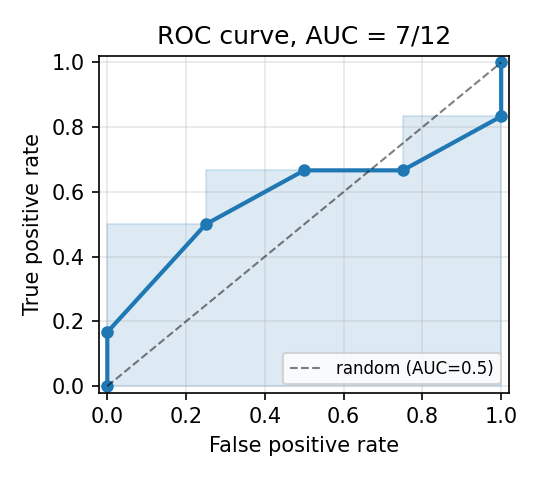
\includegraphics[width=0.42\textwidth]{q3_roc.png}
\end{figure}

AUC (trapezoid sum over FPR):
\begin{align*}
\mathrm{AUC}
&= \tfrac12\Big[\bigl(0+\tfrac16\bigr)\cdot\tfrac14
   +\bigl(\tfrac16+\tfrac12\bigr)\cdot\tfrac14
   +\bigl(\tfrac12+\tfrac23\bigr)\cdot\tfrac14
   +\bigl(\tfrac23+\tfrac23\bigr)\cdot\tfrac14
   +\bigl(\tfrac23+\tfrac56\bigr)\cdot\tfrac14 \Big] \\
&= \frac12\left[\frac{1}{24}+\frac16+\frac{7}{24}+\frac13+\frac38\right]
 = \frac{7}{12}\approx 0.5833 .
\end{align*}

% ----------------------------------------------------------------------
\section{Question 4 (20 pts)}

$lr=0.001$, $100$ epochs, init $W=\mathbf{0}$, $b=0$. Loss = average binary
cross-entropy. 2000 train samples (1000 per class), 100 test samples, 100 features,
fixed seed.

\textbf{(a)} Data: Gaussian inputs shifted to opposite sides of a random hyperplane;
noise std $0.5$ and $3\%$ label flips $\Rightarrow$ not perfectly separable.
See \texttt{A1\_Q4.py}.

\textbf{(b) GD (NumPy).}
Accuracy $=\mathbf{0.84}$. Loss: train $0.6931\to0.6700$, test $0.6931\to0.6680$.
$\lVert W\rVert_2=0.0483$, $b=0.0005$.

\textbf{(c) SGD (NumPy).}
Accuracy $=\mathbf{0.84}$. Loss: train $0.6931\to0.4219$, test $0.6931\to0.3787$.
$\lVert W\rVert_2=1.5297$, $b=0.0217$.

\textbf{(d) Loss curves:}

\begin{figure}[H]
\centering
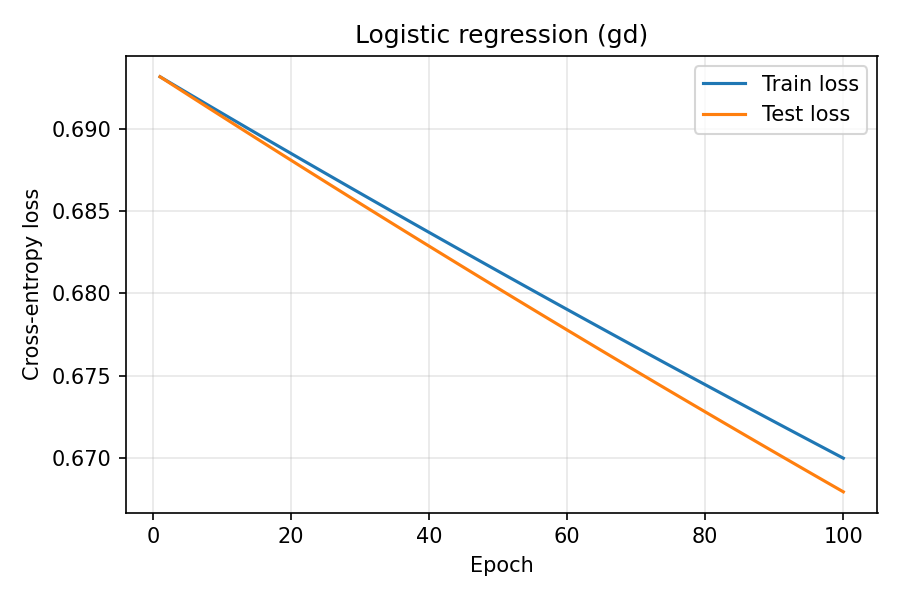
\includegraphics[width=0.45\textwidth]{gd_loss.png}\hfill
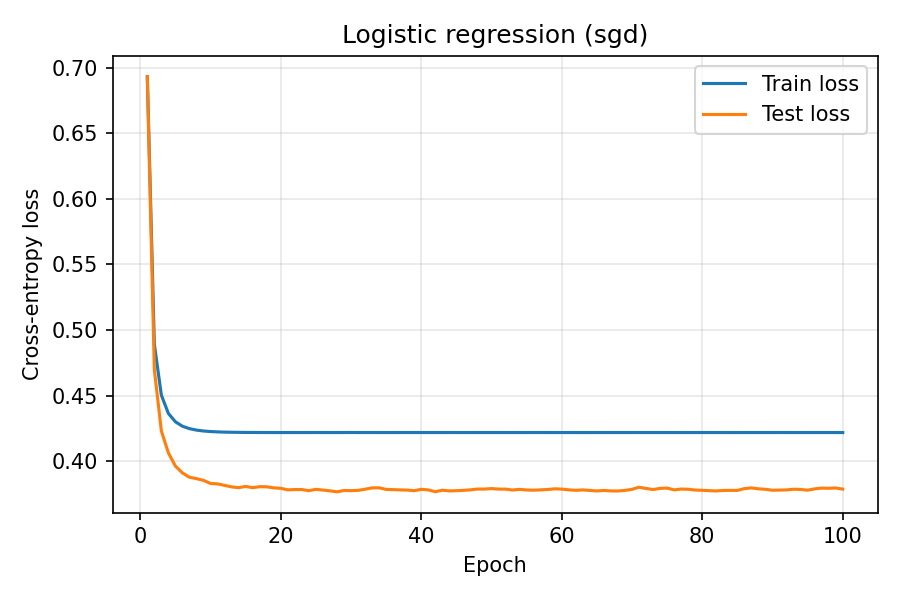
\includegraphics[width=0.45\textwidth]{sgd_loss.png}
\end{figure}

\textbf{(e) PyTorch.} \texttt{Linear(100,1)} + \texttt{Sigmoid}, \texttt{BCELoss},
\texttt{torch.optim.SGD}, no loop over samples.
Accuracy $=\mathbf{0.84}$. Loss: train $0.6931\to0.6700$, test $0.6929\to0.6677$.
$\lVert W\rVert_2=0.0483$, $b=0.0005$ (zero init $\Rightarrow$ matches GD).

\begin{figure}[H]
\centering
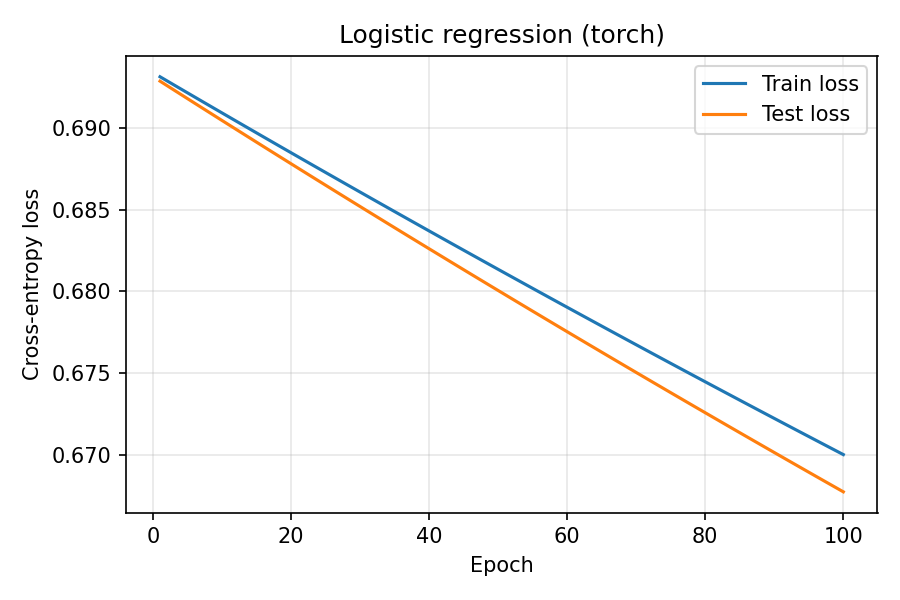
\includegraphics[width=0.45\textwidth]{torch_loss.png}
\end{figure}

% ----------------------------------------------------------------------
\section{Question 5 (10 pts)}

Iris, 105 samples, 5-fold stratified CV, standardized features.

\begin{table}[H]
\centering
\begin{tabular}{lc}
\toprule
Model & CV accuracy \\
\midrule
Logistic regression & $0.9524 \pm 0.0426$ \\
SVM (RBF)           & $\mathbf{0.9714 \pm 0.0381}$ \\
FCN $4\to64\to32\to3$ & $0.9333 \pm 0.0486$ \\
CNN (1-D)           & $0.9429 \pm 0.0356$ \\
\bottomrule
\end{tabular}
\end{table}

\textbf{Best:} SVM.

\textbf{Why no deep-network advantage:}
\begin{itemize}
  \item Only 150 samples -- too little data to estimate many parameters;
  \item Nearly linearly separable, shallow boundaries suffice -- extra depth adds
        variance, not accuracy;
  \item 4 tabular features: no spatial/hierarchical structure for convolutions or
        deep feature hierarchies to exploit.
\end{itemize}

% ----------------------------------------------------------------------
\section{Question 6 (40 pts)}

\subsection{AlexNet (ImageNet Classification with Deep CNNs)}
\textbf{Motivation:} hand-engineered features had plateaued; test whether a big,
learned deep CNN could handle ImageNet's 1.2M images / 1000 classes.
\textbf{Novelty:} first deep CNN to win ILSVRC by a large margin; ReLU, 2-GPU
training, overlapping pooling, LRN, augmentation + dropout (60M params).
\textbf{Intuition:} conv weight sharing + hierarchical features; ReLU gradients do
not vanish, so depth becomes trainable.
\textbf{Implementation:} \url{https://github.com/pytorch/vision} (AlexNet)

\subsection{ResNet (Deep Residual Learning for Image Recognition)}
\textbf{Motivation:} deeper plain nets had \emph{higher training error} --
optimization problem, not overfitting.
\textbf{Novelty:} residual learning $H(x)=F(x)+x$ via skip connections; 152 layers,
ILSVRC 2015 winner.
\textbf{Intuition:} residuals near identity are easy to learn; skips give gradients
a direct path, so extra depth only helps.
\textbf{Implementation:} \url{https://github.com/pytorch/vision} (ResNet)

\subsection{U-Net}
\textbf{Motivation:} biomedical segmentation has tiny annotated datasets; sliding
windows slow; upsampling lost detail.
\textbf{Novelty:} symmetric encoder-decoder with skip concatenations + elastic
augmentation; ISBI 2012/2015 winner.
\textbf{Intuition:} encoder gives \emph{what} (context), decoder recovers
\emph{where}; skips restore fine spatial detail.
\textbf{Implementation:}
\url{https://github.com/milesial/Pytorch-UNet}

\subsection{SimCLR}
\textbf{Motivation:} self-supervised features lagged supervised ones; prior
contrastive methods needed memory banks / special architectures.
\textbf{Novelty:} simple recipe: strong augmentation, small projection head,
NT-Xent loss, large batches; matches supervised ResNet-50 on 1\% labels.
\textbf{Intuition:} attract augmentations of the same image, repel others
$\Rightarrow$ learn nuisance-invariant semantics.
\textbf{Implementation:} \url{https://github.com/google-research/simclr}

\subsection{MAE (Masked Autoencoders)}
\textbf{Motivation:} masked prediction dominated NLP but images are too redundant
for naive reconstruction.
\textbf{Novelty:} asymmetric ViT: 75\% patches masked and removed; light decoder;
$3$-$4\times$ faster; ViT-H $87.8\%$ ImageNet.
\textbf{Intuition:} heavy masking forces semantics; discarding patches cuts compute;
decoder thrown away after pre-training.
\textbf{Implementation:}
\url{https://github.com/facebookresearch/mae}

\end{document}
